\section{Experiments}\label{sec:experiments}
In this section, we summarize our numerical experiments which verify the results from Section~\ref{sec:applications}.

% \subsection{Convergence to corrections}
% \jginline{Here we need some experiments which show that with increasing width, we converge faster to the corrected version than to the infinite-width limit}
% \jginline{One option would be to compare empirical NTKs to the mean NTK at order $\frac{1}{n}$. Interesting ablations would be width and number of ensemble members. Could use here e.g. ReLU non-single input.}
% \pminline{Unfortunately not ready yet.}

\subsection{Gradient stability}
We verify numerically for finite-width ReLU-MLPs that the preactivation and NTK statistics are stabilized for the critical initialization $C_W^{(\ell)}=C_W^\mathrm{c}=2$, whereas larger (lower) values lead to exponential growth (decay) with depth. In particular,
% To verify numerically that the forward and the backward pass can be set to criticality simultaneously, we extend the analysis found in \cite{banta2024}. They show that the empirical NNGP of a ReLU MLP stays approximately constant with depth when choosing the ReLU-specific critical value $C_W^{(l)}=C_W^\mathrm{c}=2$, whereas larger (lower) values lead to exponential growth (decay). In a similar fashion,
we compute the ensemble average \mbox{$\overline{\Theta}^{(\ell)}_{\alpha \beta} = \frac{1}{N_\mathrm{net}} \sum_{I=1}^{N_\mathrm{net}} \hat{\Theta}^{(\ell)}_{I, \alpha \beta}$} of \eqref{eq:10} for up to 30 layers to approximate the mean NTK $\Theta_{\alpha\beta}$. Here, $I$ labels the independent initializations. Figure~\ref{fig:ntk_comparison} shows the linear scaling for both the single and the distinct input case when $C_W^{(\ell)}=C_W^\mathrm{c}$, in contrast to the exponential behavior observed away from this value. In Appendix~\ref{app:experiments} we provide further details and also numerically verify the simultaneous stability of the NNGP $K$, the four-point cumulant $V_4$ and the tensors $A, B, D$ and $F$ which together describe the complete preactivation and NTK statistics up to rank four.
\begin{figure}
  \centering
  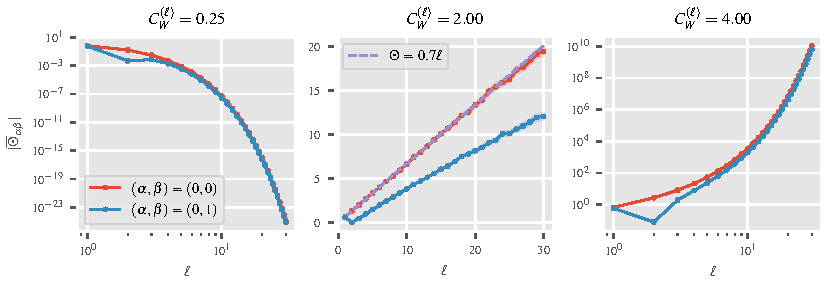
\includegraphics[width=0.95\textwidth]{figures/experiments/ntk_comparison.pdf}
  \vspace{-0.1cm}
  \caption{\emph{Gradient stability.} Components of the Monte--Carlo estimated NTK $\overline{\Theta}_{\alpha \beta}$ of a ReLU MLP as a function of layer depth $\ell$ corresponding to single and distinct inputs are shown for three different choices of $C_W^{(\ell)}$. The hidden layers are of size 200. The case for the critical value $C_W^{(\ell)} = C_W^\mathrm{c}=2$ is shown in the middle. For the single input case at criticality (red line in the middle), we also show the expected linear relation~\cite{roberts2022} (purple). Sample means are obtained from 1000 initializations. Error bands are standard errors of the mean but mostly too small to be visible.} \label{fig:ntk_comparison}
\end{figure}

\subsection{Absence of kernel-corrections for scale-invariant activations}

\begin{figure}
  \centering
  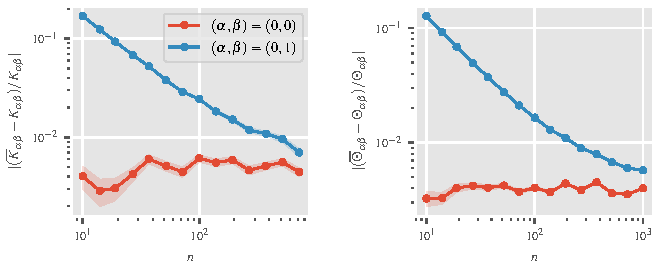
\includegraphics[width=0.75\textwidth]{figures/experiments/Relu_width_corrections_layer-4.pdf}
  \vspace{-0.1cm}
  \caption{\emph{Finite-width corrections for ReLU.} Relative deviations of the Monte--Carlo estimated NNGP and NTK to its infinite-width counterparts as a function of hidden layer width $n=n_\ell$. A four layer ReLU MLP with $C_W=2$ is sampled over $5 \times 10^6$ initializations. Error bars of the sample mean are included for all lines. Both a single and distinct input component of each kernel is shown.}\label{fig:relu_corrections}
\end{figure}

We measure the finite-width corrections to the infinite-width NTK by computing the relative deviation $|(\overline{\Theta}_{\alpha \beta} - \Theta_{\alpha \beta})/\Theta_{\alpha \beta}|$ of the ensemble average to the frozen NTK (computed with the \texttt{neural-tangents} library~\cite{novak2020a}) at different hidden-layer widths $n = n_\ell$. The NNGP corrections are investigated analogously. The results for the single and distinct input case are shown in Figure \ref{fig:relu_corrections}. Indeed, the single input component does not receive corrections, while the distinct input case only approaches the infinite-width result as $n \to \infty$.
 For further details, we refer to Appendix \ref{app:experiments}, where we also check the absence of corrections for LeakyReLU and show that the kernels do receive corrections for GeLU, which is not scale-invariant.


%%% Local Variables:
%%% mode: LaTeX
%%% TeX-master: "ntk_feynman"
%%% End:
